\chapter{Linear Perturbations}

We now drop the assumption that the universe is homogeneous and isotropic. In this chapter, we analyse small perturbations about the background, which can be handled with linear perturbation theory. These perturbations will lead to the structures that we observe today.

We are going to make a few approximations:
\begin{itemize}
	\item The perturbations are sufficiently small to be treated by linear perturbation theory.
	\item We ignore relativistic effects and use a Newtonian approximation.
\end{itemize}

There are several ways to model this structure.

\section{Ideal Fluid}
First, we model the content of the universe as an expanding, self-gravitating, ideal fluid in the Newtonian approximation. We consider the following parameters:
\begin{itemize}
	\item density $\rho(\vec{x},t)$
	\item pressure $p(\vec{x},t)$
	\item velocity $\vec{u}(\vec{x},t) = \dot{\vec{r}}$
	\item gravitational potential $\phi(\vec{x},t)$
\end{itemize}
The time evolution of these parameters is described by the \emph{fluid equations}:
\begin{align*}
	\Dv{\rho}{t} &= - \rho \Grad_r \cdot \vec{u}
	&& \text{continuity equation, conservation of mass}\\
	\Dv{\vec{u}}{t} &= - \frac{\Grad_r p}{\rho} - \Grad_r \phi
	&&\text{acceleration} = \text{pressure force} + \text{gravitational force}\\
	\Lap_r \phi &= 4 \pi G \rho
	&&\text{Poisson equation}
\end{align*}
We define the \emph{convective derivative}
\begin{align*}
	\Dv{}{t} = \pdv{}{t} + \vec{u} \cdot \Grad_r,
\end{align*}
which is the time derivative as one moves along fluid elements.

\subsection*{Assumptions}

Let's consider the case where the fluid is expanding. In order to describe this, we can write the position vector as $\vec{r} = a(t) \vec{x}$, where $\vec{x}$ is a comoving coordinate. In the Newtonian treatment, we assume that the scale factor is a known input for the calculation. Then the (total) velocity is
\begin{align*}
	\vec{u} = \dot{a}(t) \vec{x} + \vec{v},
\end{align*}
where the first term is the Hubble expansion, and $\vec{v} = a \dot{\vec{x}}$ is the peculiar velocity.

We write the density as
\begin{align*}
	\rho(\vec{x},t) = \bar{\rho}(t) [1 + \delta(\vec{x}, t)],
\end{align*}
where $\bar{\rho}(t) \propto a^{-3}$ is the mean background density, and $\delta(\vec{x}, t)$ is a small density perturbation.

We can plug these assumptions and definitions into the fluid equations to get
\begin{align*}
	\pdv{\delta}{t} + \frac{1}{a} \Div[(1+\delta)\vec{v}]
	&= 0\\
	\pdv{\vec{v}}{t} + \frac{\dot{a}}{a} \vec{v} + \frac{1}{a} [\vec{v} \cdot \Grad] \vec{v}
	&= - \frac{\Grad \Phi}{a} - \frac{\Grad p}{a \bar{\rho}(1+\delta)}\\
	\Lap \Phi
	&= 4 \pi G \bar{\rho} a^2 \delta
\end{align*}
where
\begin{align*}
	\Phi = \phi + \frac{1}{2} a \ddot{a} x^2 
\end{align*}
and $\Grad = \Grad_{\vec{x}}$.

\subsection*{Thermodynamics}

We have three equations in four unknowns, so we still need the equation of state, which relates pressure to other variables, such as density and entropy. 

The first law of thermodynamics states that internal energy can either be added by the means of heat or work:
\begin{align*}
	\dd{U} = \dd{Q} + \dd{W}
\end{align*}
We can use $\dd{W} = - p \dd{V}$ and $\dd{Q} = T \dd{S}$. From now on, we assume we are dealing with an ideal gas. The equation of state for an ideal gas is
\begin{align*}
	p
	&= n k_B T\\
	&= \frac{\rho}{\mu m_p} k_B T
\end{align*}
where $\mu$ is the mean molecular weight and $n = N/V$ is the number density. The internal energy is
\begin{align*}
	U
	&= \frac{3}{2} N k_B T\\
	&= \frac{3}{2} \frac{\rho}{\mu m_p} V k_B T
\end{align*}
Then
\begin{align*}
	\frac{\Grad p}{\bar{\rho}}
	&= \frac{1}{\bar{\rho}}
	\left[ 
		\left( \pdv{p}{\rho} \right)_S \Grad \rho
		+ 
		\left( \pdv{p}{S} \right)_\rho \Grad S
	\right]
\end{align*}
Let $c_s^2 = (\pdv*{p}{\rho})_S$ be the adiabatic sound speed squared. Then we get
\begin{align*}
	\left( \pdv{p}{S} \right)_\rho = \frac{2}{3} \rho T
\end{align*}
and thus
\begin{align*}
	\frac{\Grad p}{\bar{\rho}}
	&= c_s^2 \Grad \delta + \frac{2}{3} (1+\delta) T \Grad S
\end{align*}
The Euler equation can then be rewritten as
\begin{align*}
	\pdv{\vec{v}}{t} + \frac{\dot{a}}{a} \vec{v} + \frac{1}{a} (\vec{v} \cdot \Grad) \vec{v}
	&= - \frac{\Grad \Phi}{a} - \frac{c_s^2}{a} \frac{\Grad \delta}{1 + \delta} - \frac{2T}{3a} \Grad S
\end{align*}

\subsection*{Solving the fluid equation}

For small density perturbations $\delta$ and small peculiar velocities $\vec{v}$, we can drop terms that are quadratic in these variables, such as $(\vec{v} \cdot \Grad) \vec{v}$. We get the linearized fluid equations:
\begin{align*}
	\pdv{\delta}{t} + \frac{1}{a} \Div \vec{v} &= 0\\
	\pdv{\vec{v}}{t} + \frac{\dot{a}}{a} \vec{v} &= - \frac{\Grad \Phi}{a} - \frac{c_s^2}{a} \Grad \delta - \frac{2 \bar{T}}{3a} \Grad S
\end{align*}
We can combine them to get a single equation. First, take the derivative of the continuity equation. Then, use the Euler equation and the Poisson equation to get the following:
\begin{align*}
	\pdv[2]{\delta}{t} + 2 \frac{\dot{a}}{a} \pdv{\delta}{t} &= 4 \pi G \bar{\rho} \delta + \frac{c_s^2}{a^2} \Lap \delta + \frac{2}{3} \frac{\bar{T}}{a^2} \Lap S
\end{align*}
This is a second order differential equation. We take the Fourier transform:
\begin{align*}
	\delta(\vec{x},t) &= \sum_{\vec{k}} \delta_{\vec{k}} \exp(i \vec{k} \cdot \vec{x})\\
	\delta_{\vec{k}}(t) &= \frac{1}{V} \int \delta(\vec{x},t) \exp(-i \vec{k} \cdot \vec{x}) \dd{^3x},
\end{align*}
where $V$ is the volume of a sufficiently large box. The fluid equation then becomes\sidenote{$\Grad \to i\vec{k}$ and $\Lap \to -k^2$}
\begin{align*}
	\dv[2]{\delta_{\vec{k}}}{t} + 2 \frac{\dot{a}}{a} \dv{\delta_{\vec{k}}}{t}
	&= \left[4 \pi G \bar{\rho} - \frac{k^2 c_s^2}{a^2}\right] \delta_{\vec{k}} - \frac{2}{3} k^2 \frac{\bar{T}}{a^2} S_{\vec{k}}
\end{align*}
The Poisson equation in Fourier space is
\begin{align*}
	- k^2 \Phi_{\vec{k}} &= 4 \pi G \bar{\rho} a^2 \delta_{\vec{k}}
\end{align*}
The fluid equation can now be solved for every $\vec{k}$-mode independently.


We need initial conditions to solve the fluid equation. There are two pressure terms, $\delta_{\vec{k}}$ and $S_{\vec{k}}$. We distinguish two types of initial conditions:
\begin{itemize}
	\item $\delta \neq 0$, $\delta S = 0$: isentropic or adiabatic or curvature perturbations
	\item $\delta = 0$, $\delta S \neq 0$: isocurvature perturbations
\end{itemize}
Adiabatic perturbations are naturally generated by inflation, so we only consider those and set $\delta S = 0$.

The fluid equation can now be simplified further:
\begin{align*}
	\dv[2]{\delta_{\vec{k}}}{t} + 2 \frac{\dot{a}}{a} \dv{\delta_{\vec{k}}}{t}
	&= \left[4 \pi G \bar{\rho} - \frac{k^2 c_s^2}{a^2}\right] \delta_{\vec{k}}
\end{align*}
Consider the case where the expansion of the fluid can be ignored, so $a$ is a constant. Then $\dot{a} = 0$, so a further term drops out:
\begin{align*}
	\dv[2]{\delta_{\vec{k}}}{t}
	&= \left[4 \pi G \bar{\rho} - \frac{k^2 c_s^2}{a^2}\right] \delta_{\vec{k}}\\
	&= - \omega^2 \delta_{\vec{k}}
\end{align*}
This is simply the equation of motion of a harmonic oscillator. We can rewrite
\begin{align*}
	\omega^2
	&= \left( \frac{c_s}{a} \right)^2 [k^2 - k_J^2]
\end{align*}
where $k_J$ is the \textsc{Jeans} wavenumber
\begin{align*}
	k_J = \frac{a}{c_s} \sqrt{4 \pi G \bar{\rho}}.
\end{align*}
One can also define the Jeans wavelength
\begin{align*}
	\lambda_J = \frac{2 \pi a}{k_J},
\end{align*}
and the Jeans mass
\begin{align*}
	M_J = \frac{\pi}{6} \bar{\rho} \lambda_J^3,
\end{align*}
which is the mass of a sphere with a radius of $\lambda_J/2$ and density $\bar{\rho}$.

\subsection*{Solutions}

We first consider the case where $k > k_J$, or equivalently $\lambda < \lambda_J$, or $M < M_J$. Then $\omega^2 > 0$, and the equation of motion gives us an oscillatory solution:
\begin{align*}
	\delta_{\vec{k}} \propto \exp(\pm i \omega t)
	\qquad \omega \in \R
\end{align*}
This means that density perturbations don't grow, but just oscillate.

When $k < k_J$, the solution is
\begin{align*}
	\delta_{\vec{k}} \propto \exp(\pm \alpha t) \qquad \alpha \in \R,
\end{align*}
which indicates exponentially decaying or growing modes. The growing modes lead to the growth of structure, which is called gravitational or Jeans instability. Once the perturbations become large, our assumptions are not valid any more, and we have to switch to non-linear perturbation theory.

%In other words, either attractive gravity or repulsive pressure win in the above scenarios.

\subsection*{Jeans mass}
The Jeans mass is
\begin{align*}
	M_J
	&= \frac{\pi}{6} \bar{\rho} \lambda_J^3\\
	&= \frac{\pi^{5/2}}{6} \frac{c_s^3}{G^{3/2} \bar{\rho}^{1/2}}
\end{align*}
Before recombination, photons and baryons are tightly coupled, and they act as a single fluid. We get $M_J \approx \num{e16} (\Omega_{b,0}h^2)^{-2} M_\sol$, which means that no baryonic perturbations smaller than a supercluster can grow before recombination.

After recombination, the baryons and the photons are decoupled. They have much smaller pressure, and $M_J \approx \num{e5} (\Omega_{b,0}h^2)^{-1/2} M_\sol$. Perturbations with masses larger than a globular cluster can grow.

We also have to take into account the expansion of the universe, which we neglected up to now. Furthermore, these results do not consider dark matter, but only baryons.


\section{Collisionless gas}
We now consider a collisionless gas, such as dark matter. In this case, there is no reason to impose thermodynamic equilibrium, not even locally. As a result, we cannot describe the gas with the thermodynamic variables we used before, since they are only defined in (at least local) thermodynamic equilibrium. We thus need to take one step back and consider distribution functions $f(\vec{x}, \vec{p}, t)$, whose dynamics are given by the collisionless Boltzmann equation,
\begin{align*}
	\dv{f}{t}
	&= \pdv{f}{t} + \pdv{f}{p^i} \pdv{p^i}{t} + \pdv{f}{x^i} \pdv{x^i}{t}\\
	&= 0.
\end{align*}
As before, we can take the moments of the distribution functions:
\begin{align*}
	\langle Q \rangle = \frac{1}{n} \int \dd{^3p} Q f(\vec{x}, \vec{p}, t)
\end{align*}
with the comoving number density $n(\vec{x}, t) = \int \dd{^3p} f(\vec{x}, \vec{p}, t)$. Some moments are:
\begin{itemize}
	\item The density $\rho(\vec{x}, t)$ can be obtained with $Q = m$, where $m$ is the mass of a particle.
	\item The bulk velocity $\langle v_i \rangle$ can be obtained with $Q = v_i = p_i/(m n)$
\end{itemize}

We take moments of the Boltzmann equation. One can show that one gets the same equations as the fluid equations: the continuity equation and the Euler equation, with the pressure gradient term replaced as follows:
\begin{align*}
	\frac{\Grad_i p}{\rho}
	\to \sum_{j=1}^3 \pdv{}{x_j}
	\left[ (1+\delta) \sigma_{ij}^2 \right]
\end{align*}
where
\begin{align*}
	\sigma_{ij} = \avg{v_i v_j} - \avg{v_i} \avg{v_j}
\end{align*}
The stress tensor is defined as $\rho \sigma_{ij}^2$.

If the stress tensor is small, we get the fluid equations with $\Grad p = 0$ and $c_s^2=0$, so a pressureless fluid.

On small scales, the stress tensor can be important. The large random velocities of the particles can make these particles diffuse and dampen the perturbations. This phenomenon is called \emph{free streaming}. This is not important for cold dark matter, but it is important for hot dark matter.




\section{Solutions}

\subsection{Collisionless gas}
We assume adiabatic perturbations, neglect free streaming, and only consider cold dark matter. In the ideal fluid equations, we can set $p=0$ and $c_s^2 = 0$. We get
\begin{align*}
	\dv[2]{\delta_{\vec{k}}}{t}
	+ 2 \frac{\dot{a}}{a} \dv{\delta_{\vec{k}}}{t}
	&= 4 \pi \bar{\rho}_m \delta_{\vec{k}}
\end{align*}
We consider solutions for an expanding universe and find the following solutions (homework):
\begin{itemize}
	\item The solution $\delta_- \propto H(t)$ is decaying, since $H$ becomes smaller over time.
	\item The growing solution is
	\begin{align*}
		\delta_+ \propto H(t) \int_0^t \frac{\dd{t'}}{a(t)^2 H(t')},
	\end{align*}
	which is a result of gravitational instability. This is similar to what we found before, but this time we did not neglect expansion. We define $D(z) \propto \delta_+$ the linear growth factor.
\end{itemize}

\begin{figure}
	\centering
	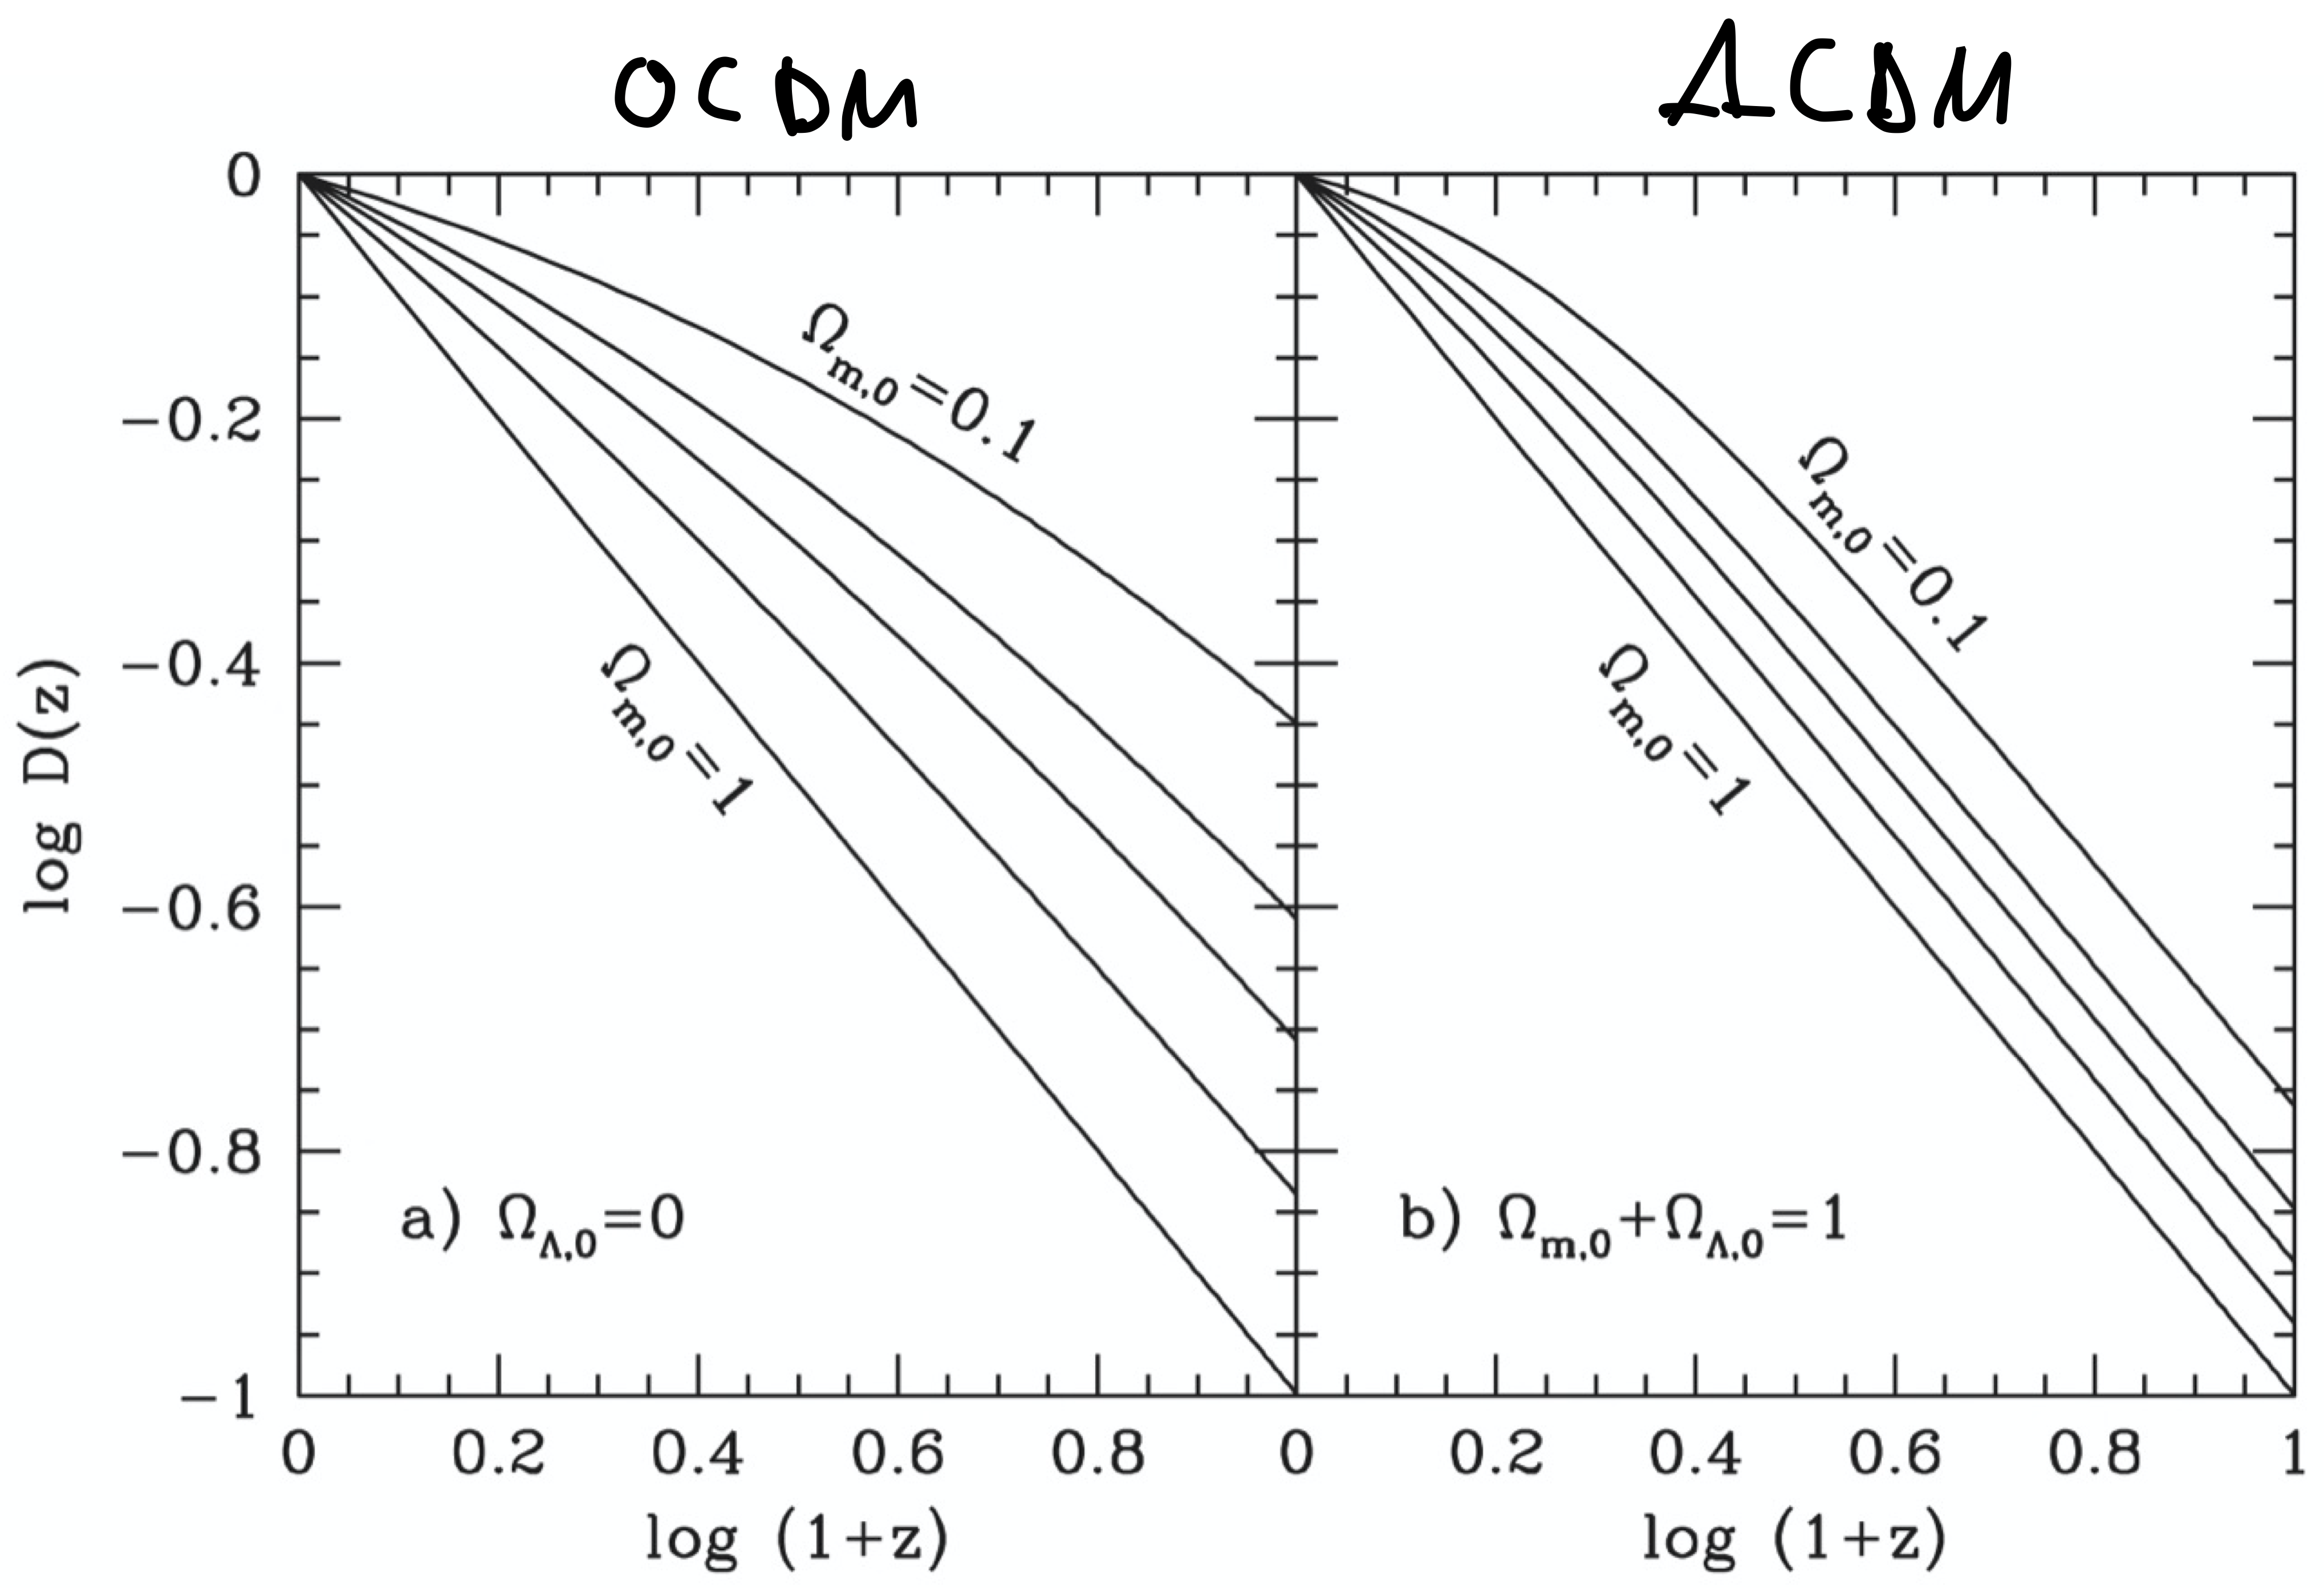
\includegraphics[width=\textwidth]{img/ch-03/collisionless-gas.png}
	\caption{Collisionless gas}
	\label{fig:collisionless-gas}
\end{figure}

Examples are shown in \cref{fig:collisionless-gas}.
\begin{itemize}
	\item Matter dominated case ($\Omega_0 = \Omega_{m,0} = 1$): $a \propto t^{2/3}$ and $H \propto t^{-1}$. This yields
	\begin{align*}
		D \propto t^{2/3} \propto a
	\end{align*}
	\item OCDM ($\Omega_{m,0} < 1$, $\Omega_{\Lambda,0} = 0$) and ΛCDM ($\Omega_{m,0} + \Omega_{\Lambda,0} = 1$): We get an analytical solution where $D$ grows slower than $a$. The faster expansion from ΛCDM slows down the growth of structure.
	\item In the general case, there is no analytical solution. The growth factor usually grows slower than the exponential growth we found in the non-expanding gravitational instability case. In other words, the universe expansion slows down with the growth of structure.
\end{itemize}



Let's look at how the gravitational potential grows, because we will need that result later. The Poisson equation in Fourier space is
\begin{align*}
	- k^2 \Phi_{\vec{k}} = 4 \pi G \bar{\rho} \delta_{\vec{k}},
\end{align*}
which can be rearranged to
\begin{align*}
	\Phi_{\vec{k}}
	&\propto a^2 \bar{\rho}_m \delta_{\vec{k}}\\
	&\propto a^2 a^{-3} D(a) \\
	&\propto \frac{D(a)}{a}
\end{align*}
This means that $\Phi_{\vec{k}}$ is constant in the matter dominated case, and $\Phi_{\vec{k}}$ decays in the OCDM and ΛCDM cases at late times.


\subsection{Two non-relativistic components}
We consider collisionless dark matter and collisionfull baryons. We assume that the pressureless dark matter dominates the matter density, so $\rho_\text{tot} \approx \rho_\text{dm}$.

There are now two differential equations:
\begin{align*}
	\dv[2]{\delta_{\text{dm}, \vec{k}}}{t}
	+ 2 \frac{\dot{a}}{a} \dv{\delta_{\text{dm}, \vec{k}}}{t}
	&= 4 \pi G \bar{\rho}_m \delta_{\text{dm}, \vec{k}}\\
	\dv[2]{\delta_{\text{b}, \vec{k}}}{t}
	+ 2 \frac{\dot{a}}{a} \dv{\delta_{\text{b}, \vec{k}}}{t}
	+ \frac{k^2 c_s^2}{a^2} \delta_{\text{b},\vec{k}}
	&= 4 \pi G \bar{\rho}_m \delta_{\text{dm}, \vec{k}}
\end{align*}
The first equation is the same as in the previous section, because the low-density baryons don't influence the dark matter much. To get analytical solutions, we assume that we are in the matter dominated case, and that $c_s^2 a$ is constant.\sidenote{The latter is equivalent to the condition that the baryons are a specific kind of polytropic fluid, which obeys $p \propto \rho^{4/3}$. For different polytropic indices $\gamma \neq 4/3$, the behaviour is similar, but the equations have to be solved numerically.}

Since the dark matter equation is the same, it has the same solution, with a growing mode $D(t) \propto a$ in a matter dominated universe.

For the baryons
\begin{align*}
	\delta_{\text{b},\vec{k}}(t)
	&= \frac{\delta_{\text{dm},\vec{k}}(t)}{1 + (k/k_J)^2},
\end{align*}
where $k_J = a/c_s \sqrt{4 \pi G \bar{\rho}}$ is the Jeans wavenumber. From this equation, we see that the baryon perturbations are equal to the dark matter perturbations for small $k$. For large $k$, pressure becomes more important, and the baryon perturbations will be smaller.\sidenote{Keep in mind that large $k$ means small length scales, and vice versa. When particles are close together, pressure becomes important.}

\paragraph*{Acoustic oscillations}
We have just seen that baryon behaviour becomes a lot more interesting at smaller length scales, where pressure is higher. This leads to oscillations and damping of the amplitude of the perturbations. One can show that the baryon density of a given mode $\vec{k}$ oscillates like
\begin{align*}
	\delta_{\text{b},\vec{k}} \propto \exp(\frac{i k c_s t}{a}) + \text{constant},
\end{align*}
which corresponds to sound waves, which is why they are called \emph{acoustic oscillations}.


\paragraph*{Collisional damping}
Before recombination on small scales, the perturbations are damped by imperfect coupling between baryons and photons. This leads to diffusion of the photons, which suppresses perturbations on small scales. The effect is called \emph{collisional damping} or \emph{Silk}\sidenote{After Joseph Silk, who first discussed photon diffusion in a paper in 1968.} \emph{damping}.



\section{Relativistic perturbations}
For a full treatment of cosmological perturbations, we need a relativistic treatment. We will only give a sketch of the formalism here.

The Einstein equations give the time evolution of space-time. The perturbed version of these equations is
\begin{align*}
	\bar{G}_{\mu\nu} + \delta G_{\mu\nu} = 8 \pi G (\bar{T}_{\mu\nu} + \delta T_{\mu\nu}),
\end{align*}
where the variables with a bar are the background solutions from the FRW metric, and the $\delta$-terms are sufficiently small perturbations, so that we can treat them with linear perturbation theory.

In order to calculate $G$, we need a metric, which we assume to be of the form
\begin{align*}
	g_{\mu \nu} = \bar{g}_{\mu\nu} + h_{\mu\nu},
\end{align*}
where $\bar{g}$ is the FRW metric, and $h$ is a again a small perturbation.
The perturbation $h$ can again be decomposed, according to the behaviour of their components under coordinate changes.
\begin{itemize}
	\item Tensor perturbations correspond to gravitational waves, which are important for the polarization of the CMB. However, they are too small to have been detected directly from the CMB.
	\item Vector perturbations are vorticity modes, which decay. They are thus not very important in cosmology.
	\item Scalar perturbations can be thought of perturbations in the gravitational potential. They play a central role in structure formation, so we will focus solely on them.
\end{itemize}

The stress energy tensor can be related to the distribution function of different components $i$ of the universe,
\begin{align*}
	T_{\mu\nu} &= \sum_{i} T^{i}_{\mu\nu}\\
	T^{i}_{\mu\nu} &= \int \frac{\dd{^3p}}{(2\pi)^3 E} p_\mu p_\nu f^i(\vec{x},\vec{p},t),
\end{align*}
where $f$ can be found from the Boltzmann equation. The distribution function can also be spilt into a background and a small perturbation:
\begin{align*}
	f^i = \bar{f}^i + \delta f^i.
\end{align*}
These species $i$ are dark matter, baryons, photons, neutrinos, and potentials of the metric perturbations. We only consider scalar perturbations. All these species interact with each other:
\begin{itemize}
	\item All species interact with the metric.
	\item Photons and electrons interact through Compton scattering.
	\item Electrons and protons interact through Coulomb scattering.
\end{itemize}
Other forces, such as the weak interaction, are neglected, since they are too rare or weak.

The resulting set of linear differential equations are called the \emph{linearised Einstein-Boltzmann equations}. They have no analytical solution in general, but there are analytical solutions in asymptotic limits.

\subsection*{Solutions in asymptotic limits}
For each $\vec{k}$ mode, the equations can be solved separately. There are several important scales:
\begin{itemize}
	\item $k^{-1}$ is the comoving wavelength scale of the $\vec{k}$-mode
	\item $\chi_h$ is the comoving horizon
	\item $a_\text{eq}$ is the scale factor at matter-radiation equality, or $a_{\text{eq2}}$ at matter-dark energy equality
	\item $\chi_h(a_\text{eq})$ is the size of the horizon at matter-radiation equality
\end{itemize}

\begin{figure}
	\centering
	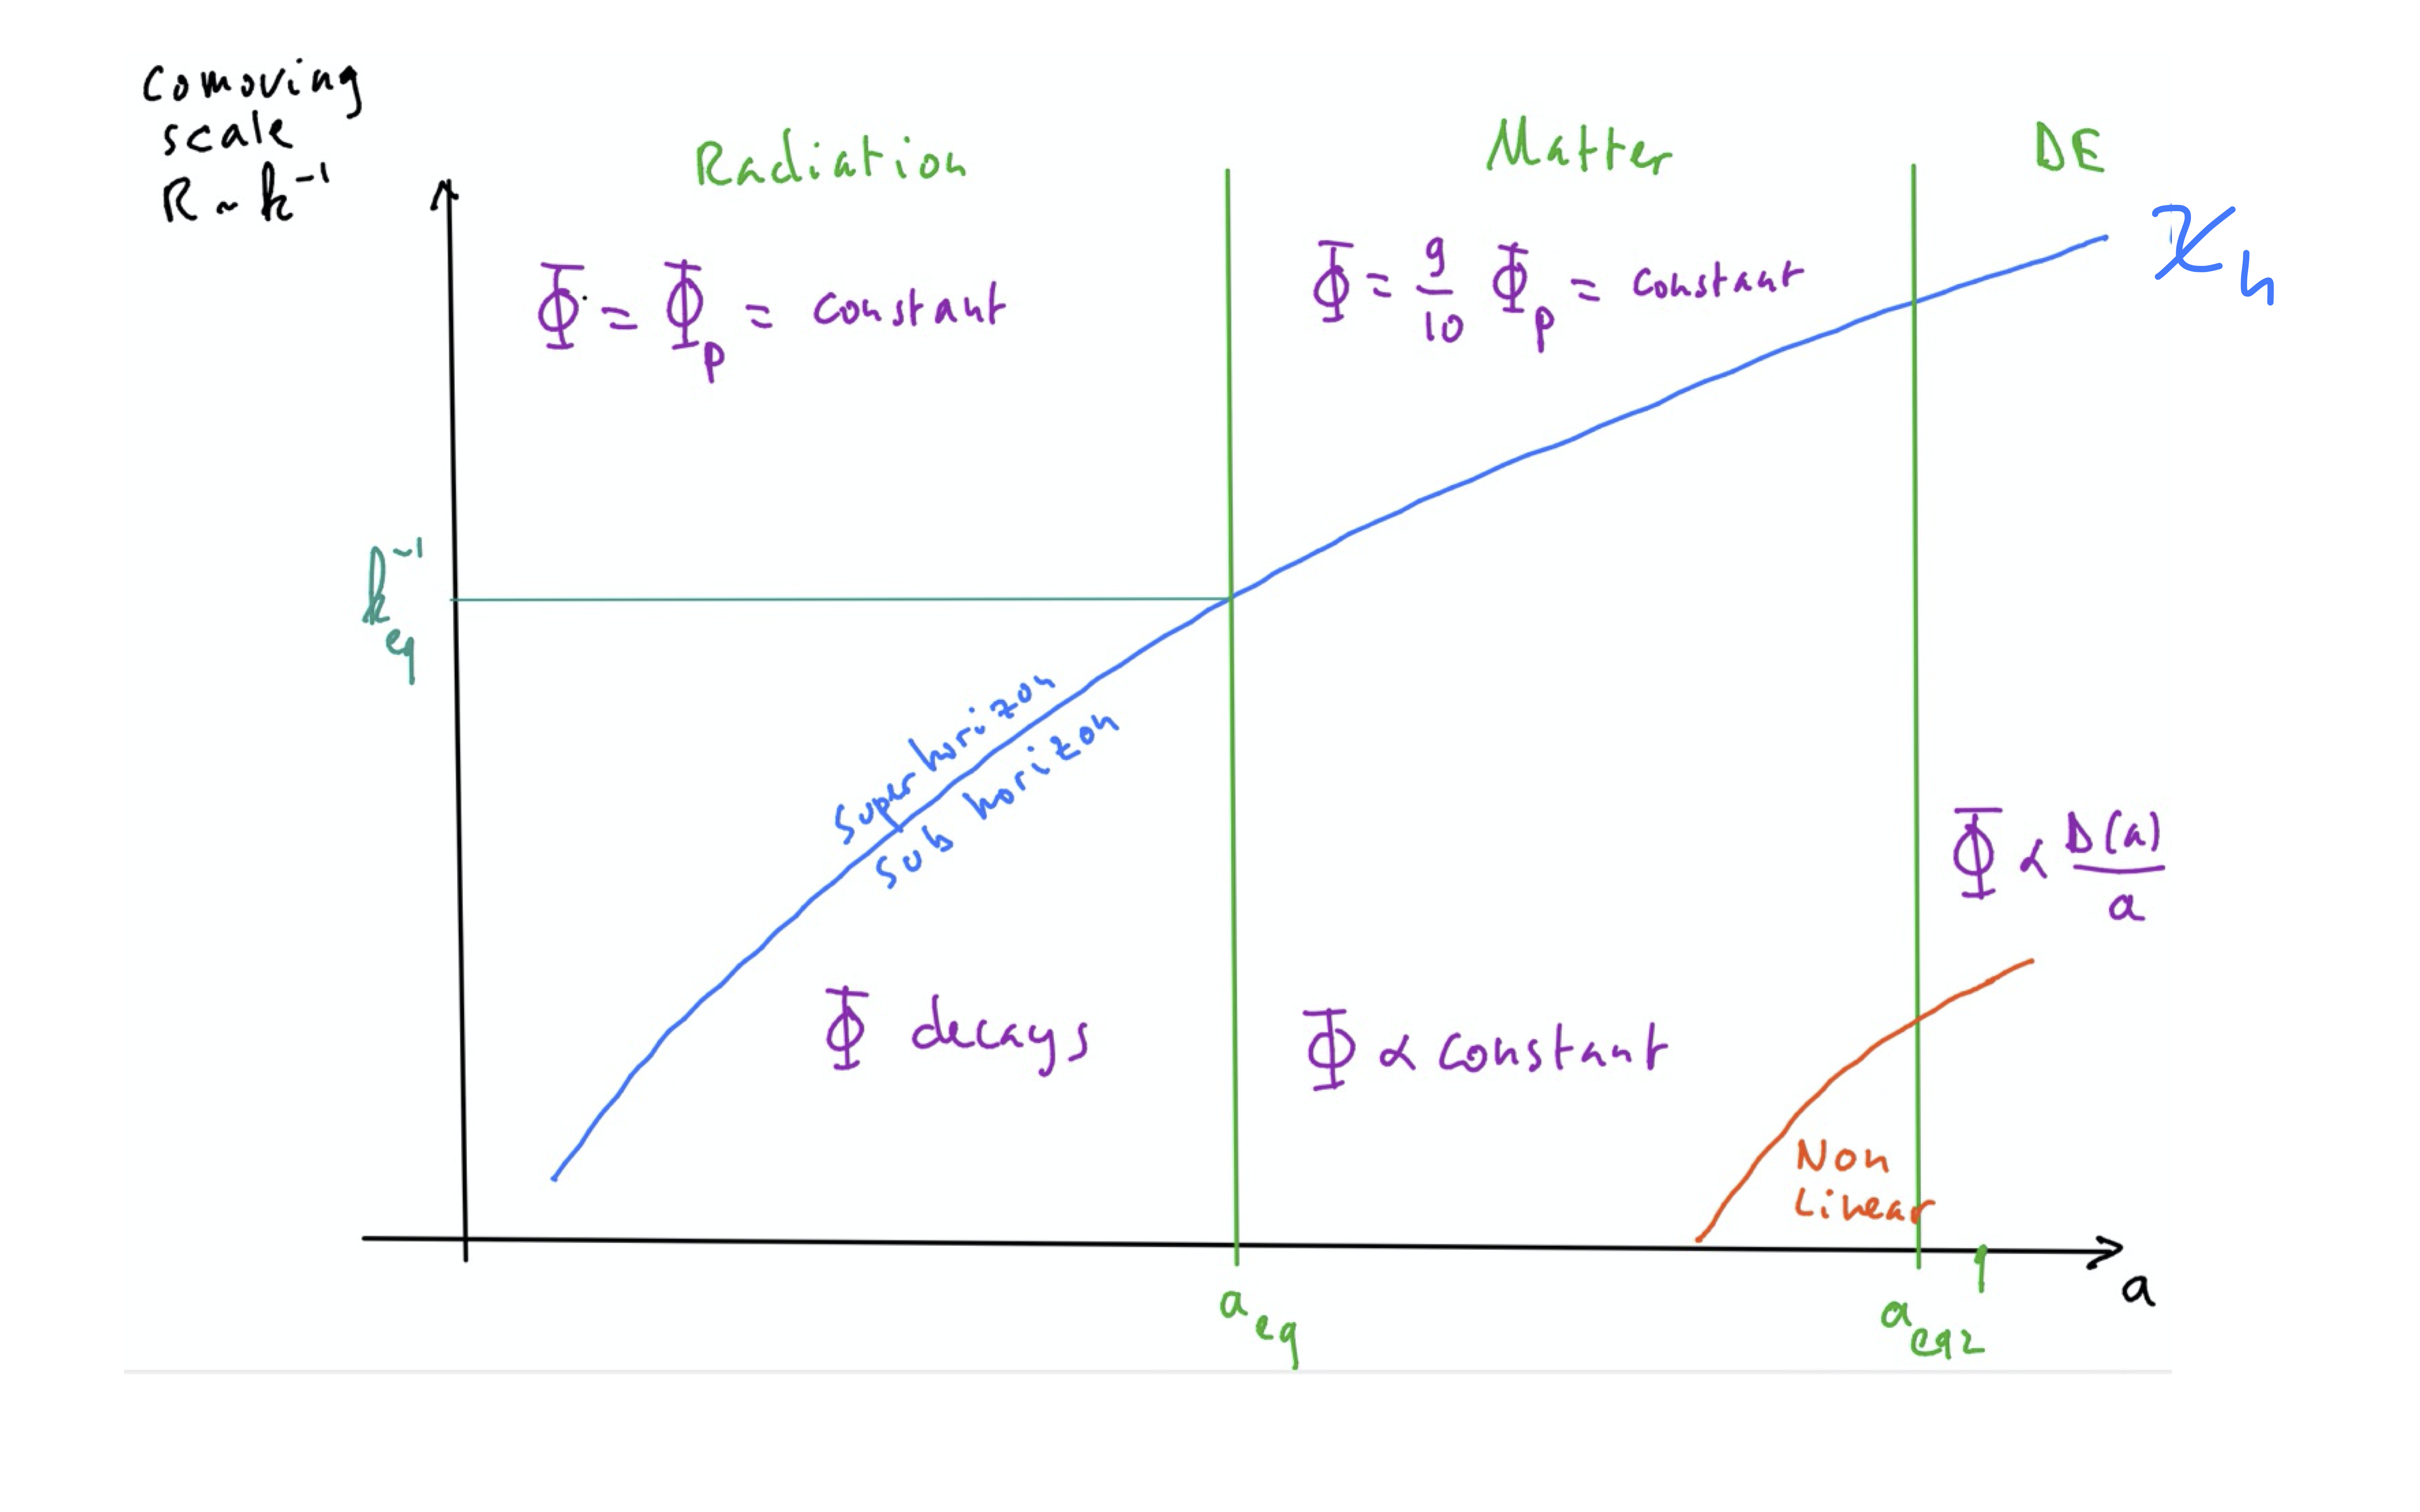
\includegraphics[width=\textwidth]{img/ch-03/asymptotic-behaviour.png}
	\caption{Solutions in asymptotic limits. Time is represented by $a$ on the horizontal axis, with early times on the left and today on the right. The cosmological eras are separated by green lines. The comoving wavelength $k^{-1}$ is shown on the vertical axis. The horizon scale $\chi$ (blue) determines whether the scale of a mode is inside (sub-horizon) or outside the horizon (superhorizon). As time increases, larger modes enter the horizon. At late time, small modes become non-linear.}
	\label{fig:asymptotic-behaviour}
\end{figure}

The solution of the Einstein-Boltzmann equations is the potential $\Phi$, shown in \cref{fig:asymptotic-behaviour}. We consider the evolution of a very large and a very small mode:
\begin{itemize}
	\item Large modes ($k \ll k_\text{eq}$) are constant in the radiation era. When entering the matter era, they lose about \SI{10}{\percent} of their amplitude, but then remain constant.
	\item Small modes ($k\gg k_\text{eq}$) decay in the radiation era, but remain constant in the matter era. In the dark energy era, they evolve as $D(a)/a$, which we have already seen in the Newtonian treatment.
\end{itemize}
In summary, small modes are suppressed, while large modes stay mostly constant.



\section{Transfer function}
We can describe the transition from early times to the matter dominated era by a \emph{transfer function}. We write the potential at late times ($a \gg a_\text{eq}$) as
\begin{align*}
	\Phi_k(a) = \frac{9}{10} \Phi_{p, k} T(k) \frac{D(a)}{a}
\end{align*}
\begin{itemize}
	\item $\Phi_{p, k}$ is the primordial potential, which is the potential at initial conditions.
	\item $T(k)$ is the transfer functions, which obeys $T \to 1$ as $k \to 0$
	\item $D(a)$ is the growth factor, normalized such that $D(a) = a$ in the matter era.\sidenote{We have derived $D(a) \propto a$ before, so we can do this.}
	\item The $9/10$ factor is the large scale suppression which we have seen in the previous diagram.
\end{itemize}
The transfer function describes how much of the primordial potential is still left at a time corresponding to scale factor $a$.
The solution for different cases is shown in \cref{fig:transfer-function}.
\begin{figure}
	\centering
	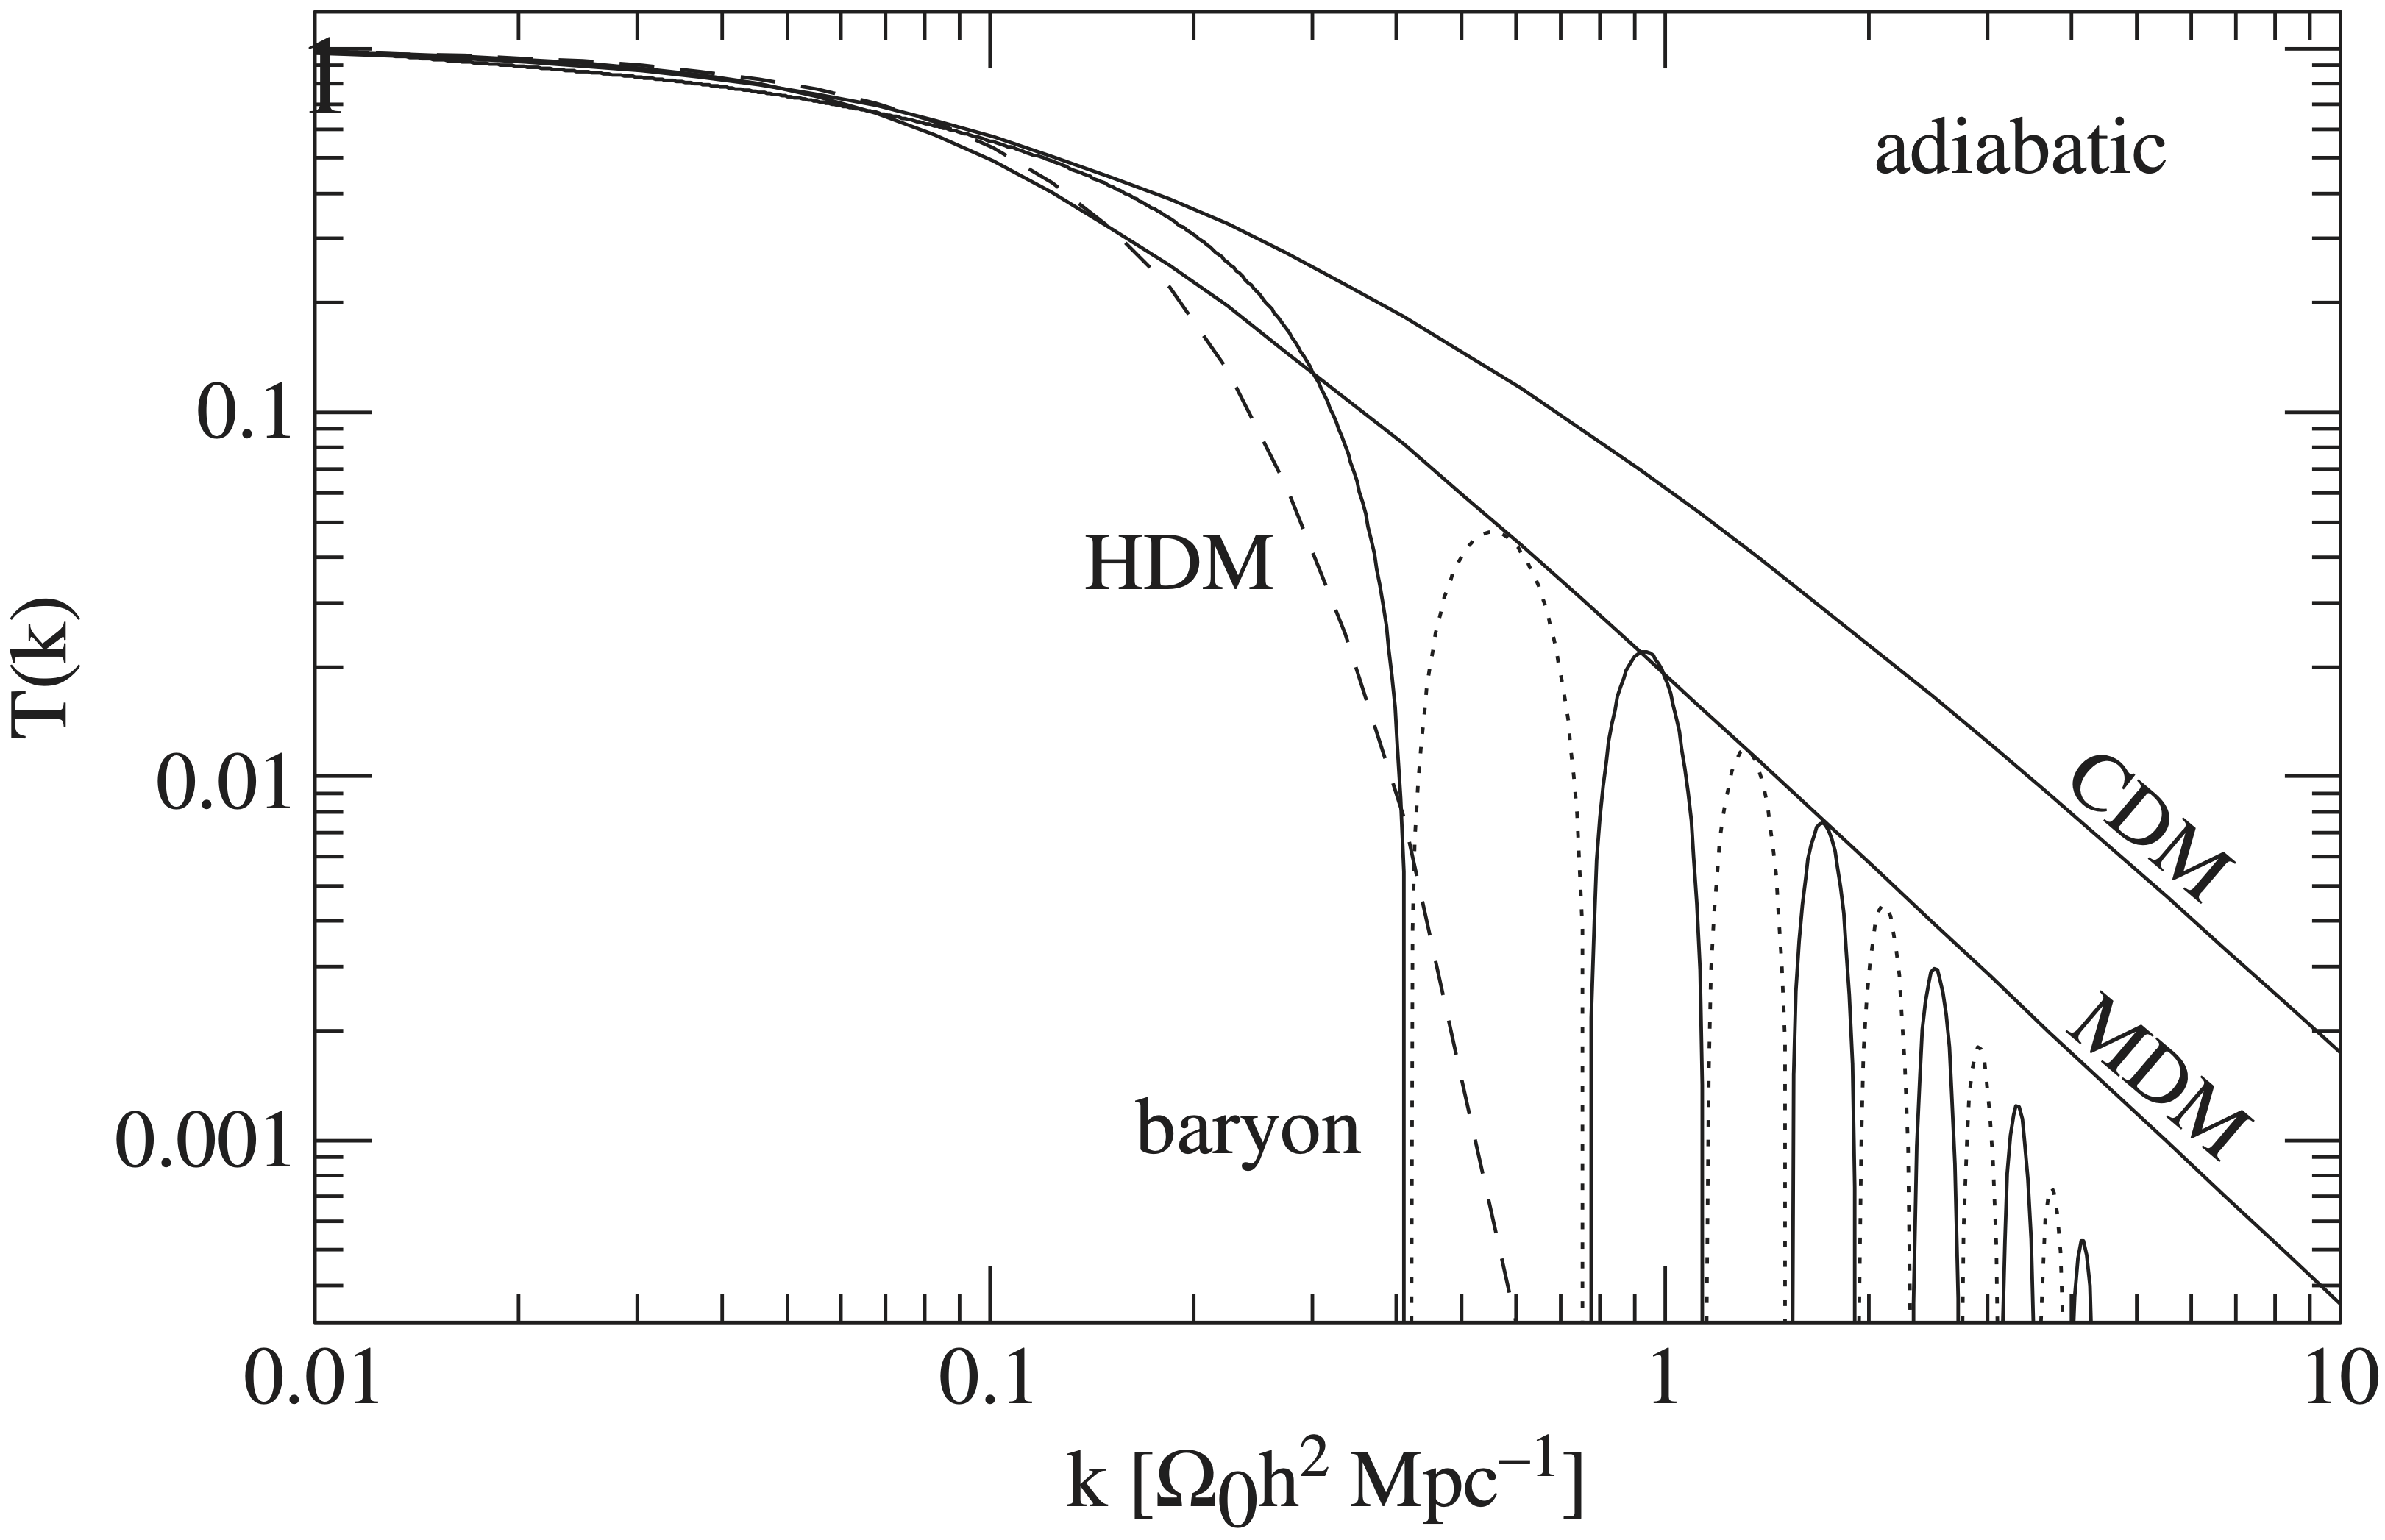
\includegraphics[width=\textwidth]{img/ch-03/transfer-function.png}
	\caption{The transfer function for adiabatic perturbations. Results are shown for a purely baryonic model, for a cold dark matter model, a hot dark matter model, and a mixed dark matter model. The dotted parts indicate negative values.}
	\label{fig:transfer-function}
\end{figure}

At small $k$, $T = 1$ as required.
\begin{itemize}
	\item In the CDM model, $T(k)$ is suppressed at $k \gg k_\text{eq}$, as we have seen before. We find $T(k) \propto (k/k_\text{eq})^2 \ln(k/k_\text{eq})$.
	\item In the HDM model\sidenote{For example, dark matter which is made up of neutrinos}, the perturbations are damped strongly due to free streaming when $k > k_\nu$.
	\item In the baryon model, dark matter is made up of baryons, which is ruled out for different reasons, but we can still look at the solution. Here, two processes act in addition to $k_\text{eq}^{-1}$ suppression:
	\begin{itemize}
		\item Jeans instability for $k > k_J$ inhabits growth, and instead leads to oscillations. We have seen these as oscillations in time at constant $k$ before, while here they are shown as oscillations in $k$ at constant time.
		\item Silk damping.
	\end{itemize}
	As a result, $T(k)$ is suppressed and oscillates on small scales.
	\item In a mixed model\sidenote{\SI{70}{\percent} CDM and \SI{30}{\percent} HDM}, nothing very interesting happens.
	\item In CDM + baryons (blue line), small oscillations occur around the CDM curve.
\end{itemize}



\section{Primordial perturbations}
Inflation also gives a mechanism to generate primordial perturbations. Remember that we proposed an inflaton field $\phi$, which is in a false vacuum configuration at the beginning, leading to vacuum energy. This drives an accelerated expansion. We required that the scale factor grew by $a_e/a_i > e^{60}$ during inflation, so small features are blown up to macroscopic features. These act as the initial perturbations for formations of structure.

The quantum harmonic oscillator is described by the Hamiltonian
\begin{align*}
	H = \frac{p^2}{2m} + \frac{1}{2} m \omega^2 x^2,
\end{align*}
which gives rise to equally spaced energy levels
\begin{align*}
	E_n = \frac{\hbar}{m \omega}
	\left( m + \frac{1}{2} \right),
\end{align*}
for $n \in \set{0, 1, 2, \dots}$. We consider a state $\ket{n}$, which deviates from its average position by
\begin{align*}
	\expval{x^2} = \expval{x^2}{n}
	= \frac{\hbar}{m\omega}
	\left( n + \frac{1}{2} \right).
\end{align*}
We can see that even for the ground state $n=0$, fluctuations exist. For inflation, each $\vec{k}$-mode $\Phi_{\text{p},\vec{k}}$ acts like a quantum harmonic oscillator.

We define the power spectrum\sidenote{What this means is explained in the next section.} as the second moment of the Fourier-transformed primordial potential, $P(k) \propto \langle{\abs{\Phi_{\vec{p},k}}^2}\rangle$. One can show that $P(k) \propto k^{n-4}$, where $n$ is arbitrarily close to $1$, and depends on the slow roll parameters $\dv*{V}{\phi}$ and $\dv*[2]{V}{\phi}$. The case $n=1$ is called \emph{scale invariant} or \emph{Harison-Zel'dovich}.

Inflation generically predicts the following:
\begin{itemize}
	\item The perturbations are adiabatic, which was explained in the previous chapter.
	\item The perturbations are Gaussian, which will be explained in the next section.
\end{itemize}




\section{Cosmological field statistics}
The density contrast $\delta(\vec{x}, t)$ can be measured more-or-less accurately by observations. We can also get a simulated density contrast from a model. There is, however, a problem when trying to compare the measurements with the prediction of the model, since we are attempting to compare two different realizations of a random quantum process. 

One way to solve this problem is to compare not the particular density contrasts, but the underlying probability distributions. For a given model, these do not suffer from any randomness, and can therefore be compared directly.

We divide the universe into $n$ cells, which are centred at positions $\vec{x}_1, \dots, \vec{x}_n$. The random perturbation field is then characterized by the probability distribution function,
\begin{align*}
	\Prob_x(\delta_1, \dots, \delta_n) \dd{\delta_1} \cdots \dd{\delta_n},
\end{align*}
which is the probability that the field $\delta$ has values in the range $\delta_i$ to $\delta_i + \dd{\delta_i}$ at positions $\vec{x}_i$.

As we see, this function $\Prob_x$ could be very complicated, potentially taking a huge number of arguments as input. To simplify the situation, we look only at some statistical moments of $\Prob_x$.

\subsection{Statistical moments}
A statistical moment is a quantity that describes the shape of a function. If the function is a probability distribution, some well-known examples of moments are the expected value and the variance.

The moments of a probability distribution $\Prob_x$ are defined as\sidenote{If this looks unfamiliar, compare it with the notation that is used in mathematics for the $n$-th moment $\mu_n$ of a single-variate probability distribution $P$,
\begin{align*}
	\mu_n = \int x^n P(x) \dd{x}.
\end{align*}}
\begin{align*}
	\moment{\delta_1^{\ell_1} \dots \delta_n^{\ell_n}}
	&= \int \delta_1^{\ell_1} \cdots \delta_n^{\ell_n}
	\Prob_x(\delta_1, \dots, \delta_n) \dd{\delta_1} \cdots \dd{\delta_n},
\end{align*}
where $\ell_i \in \set{0, 1, 2, \dots}$. Because of the cosmological principle, all moments are invariant under spatial translation and rotation.

The first moment is the expected value, $\moment{\delta} = 0$, because the density distribution is expected to be zero by assumption.\sidenote{Compare this with a perhaps more familiar notation of the expected value, $\mu = \int x P(x) \dd{x}$.}

Some more moments are the variance $\sigma^2 = \moment{\delta^2}$, and the two-point correlation function
\begin{align*}
	\xi(x) = \moment{\delta_1 \delta_2}, \quad \text{with } x = \abs{\vec{x}_1 - \vec{x}_2}.
\end{align*}
Note that $\xi(0) = \sigma^2$, and that $\xi(x)$ only depends on the distance between $\vec{x}_1$ and $\vec{x}_2$.

The same analysis can be performed in Fourier space,\sidenote{Remember our convention for the Fourier transform,
\begin{align*}
	\delta(\vec{x},t)
	&= \sum_{\vec{k}} \delta_{\vec{k}}(t) \exp(i \vec{k} \cdot \vec{x})\\
	\delta_{\vec{k}}(t) &= \frac{1}{V} \int \delta(\vec{x},t) \exp(-i\vec{k}\cdot\vec{x}) \dd{^3\vec{x}}.
\end{align*}
Also, be aware that we have to convert the probability distribution to Fourier space, written as $\Prob_k$.}
where we define the power spectrum,
\begin{align*}
	P(k)
	&\defeq V \moment{\abs{\delta_k}^2},
\end{align*}
which is the variance in Fourier space. It can be related to the two-point correlation function:
\begin{align*}
	P(k)
	&= \int \xi(\abs{\vec{x}}) \exp(-i\vec{k}\cdot\vec{x}) \dd{^3 \vec{x}},\\
	\xi(r)
	&= \frac{1}{(2\pi)^3} \int P(k) \exp(i \vec{k}\cdot\vec{r}) \dd{^3\vec{k}}.
\end{align*}
	
The variance in position space can then be written in terms of the power function,
\begin{align*}
	\moment{\delta^2}
	&= \frac{1}{(2\pi)^3} \int P(k) \dd{^3\vec{k}}\\
	&= \frac{1}{2\pi^2} \int P(k) k^2 \dd{k}\\
	&= \frac{1}{2\pi^2} \int P(k) k^3 \dd{\ln(k)}.
\end{align*}
We define $\Delta^2(k) = k^3 P(k)/2\pi^2$, which is the contribution to the variance per $\ln(k)$ interval.

\subsection{Smoothing}
If we only want to analyse features larger than a certain size limit, we convolve the density contrast with a smoothing kernel. An example for such a kernel is the top hat sphere,
\begin{align*}
	W_R(r) = 
	\begin{cases}
	\frac{3}{4\pi R^3} & \text{if } r \leq R,\\
	0 & \text{otherwise}.
	\end{cases}
\end{align*}
The smoothed field $\delta_R$ is then defined as a convolution of the original field and the kernel:
\begin{align*}
	\delta_R(\vec{x},t)
	&= \int \dd{^3 \vec{y}} \delta(\vec{y},t) W_R(\vec{x}-\vec{y}),
\end{align*}
which is commonly written $\delta_R = \delta \convolve W_R$.

The variance of the smoothed field is then\sidenote{We can simplify the calculation by using the convolution theorem,
\begin{align*}
	\widetilde{f \convolve g} &= \widetilde{f} \cdot \widetilde{g},\\
	\widetilde{f \cdot g} &= \widetilde{f} \convolve \widetilde{g}.
\end{align*}}
\begin{align*}
	\moment{\delta_R^2}
	&= \frac{1}{2 \pi^2} \int P(k) \widetilde{W}_R^2 k^2 \dd{k},
\end{align*}
where $\widetilde{W}_R$ is the Fourier transform of $W_R$, which is
\begin{align*}
	\widetilde{W}_R(k)
	&= \frac{3}{k R^2} [\sin(kR) - kR \cos(kR)].
\end{align*}

\subsection{Gaussian fields}

The probability distribution can be fully recovered if all of its statistical moments are known, as long as the distribution is homogeneous and isotropic. \emph{Gaussian fields}, where $\Prob(\delta(\vec{x}_1) \cdots \delta(\vec{x}_n))$ is proportional to a multivariate Gaussian function, can still be fully recovered if only the two-point correlation function is known. Consequently, higher order moments can be expressed in terms of the two-point correlation function.

In the standard model of cosmology, we assume that the perturbation fields are initially Gaussian, but they can evolve to non-Gaussian fields later. Then, the initial power spectrum of the perturbation field is all we need to know to fully characterize the field.




\section{Matter power spectrum}
We can now combine the results of the previous three sections.
The Poisson equation is
\begin{align*}
	- k^2 \Phi_{\vec{k}}(a)
	&= 4 \pi G \bar{\rho}_\text{m} a^2 \delta_{\vec{k}}(a),
\end{align*}
which can be rearranged and combined with the definition of the transfer function to
\begin{align*}
	\delta_{\vec{k}}(a)
	&= \frac{2}{5} \frac{k^2}{\Omega_m H_0^2} \Phi_{p, \vec{k}} T(k) D(a),
\end{align*}
where $a \gg a_\text{eq}$, as we required when we introduced the transfer function.
The primordial power spectrum obeys $P(k) \propto k^{n-4}$, and it is commonly written as
\begin{align*}
	P_{\Phi_p}(k) = \frac{50 \pi^2}{9 k^3} 
	\left( \frac{k}{H_0} \right)^{n-1}
	\delta_{H}^2 
	\left( \frac{\Omega_m}{D(a=1)} \right)^2,
\end{align*}
where $\delta_H$ is a normalization parameter.\sidenote{The normalization can be done in two ways:
\begin{itemize}
	\item With $\delta_H$, convenient to relate to the CMB anisotropy power spectrum
	\item With $\sigma_8$, equal to $\sigma_R$ with $R = 8 h^{-1} \si{\mega\parsec}$ at $z=0$. This is convenient for large scale structure measurements at low redshifts.
\end{itemize}}
Combining all these, we get
\begin{align*}
	P(k,a)
	&= V \moment{\abs{\delta(k,a)}^2}\\
	&= 2 \pi^2 \delta_H^2 
	\frac{k^n}{H_0^{n+3}}
	T(k)^2
	\left( \frac{D(a)}{D(a=1)} \right)^2.
\end{align*}

The matter power spectrum is plotted as a function of $k$ for different cosmological models in \cref{fig:matter-power}.
\begin{itemize}
	\item In the ΛCDM model, the turnover is at $k_\text{eq} \propto \Omega_m h^2$.
	\item In the SCDM model (no cosmological constant, compensated with larger $\Omega_m$), the turnover is at a higher $k$.
	\item In the HDM model, free streaming suppresses perturbations on small scales, so the power at large $k$ falls off quickly.
\end{itemize}
As we can see, by measuring the power spectrum on small scales, we can distinguish the models fairly well.

% TODO
% \begin{figure}
% 	\centering
% 	\includegraphics[width=\textwidth]{img/ch-03/matter-power.png}
% 	\caption{Matter power spectrum}
% 	\label{fig:matter-power}
% \end{figure}

We look at the matter power spectrum for ΛCDM in more detail in \cref{fig:power-lcdm}. 

% TODO
% \begin{figure}
% 	\centering
% 	\includegraphics[width=\textwidth]{img/ch-03/power-lcdm.png}
% 	\caption{Matter power spectrum for ΛCDM. Redshift $z$ is a proy for time, with $z=0$ on top and $z=2$ on the bottom.}
% 	\label{fig:power-lcdm}
% \end{figure}

\begin{itemize}
	\item At large scales, $P(k) \propto k^n$, which is essentially the same as the primordial power spectrum.
	\item The peak is at $k_\text{eq} \approx \SI{0.0073}{\per\mega\parsec} \Omega_m h^2$.
	\item At intermediate scales, there are baryon acoustic oscillations (BAO). These are at a scale of \SI{0.04}{\per\mega\parsec}, corresponding to a size of the horizon of \SI{150}{\mega\parsec}, which is called the sound horizon.
	\item At small scales,
	\begin{align*}
		P(k)
		&\propto k^n T(k)^2\\
		&\propto k^{n-4} \ln
		\left( \frac{k}{k_\text{eq}} \right)^2
	\end{align*}
\end{itemize}
At small scales, the amplitude of the perturbations become large, and the linear model no longer holds. As a result, $P(k)$ needs non-linear corrections. We define $k_\text{NL}$ such that $\Delta(k_\text{NL})^2 = 1$. We find that $k_\text{NL}$ decreases as $t$ increases, so small scales become non-linear first, and large scales later. Small objects form earlier, and large objects form later by merging of smaller ones. This is called a \emph{hierarchical model} for structure formation.
 
First, galaxies, and then groups were starting to form.
Today, galaxy clusters, with a mass of $\num{e14} M_\sol$, are starting to form.
Superclusters are not collapsing yet, but should do so later.






\section{Cosmic Microwave Background anisotropies}
Remember that the CMB gives us a picture of the universe at last scattering, which happened at $z_* \approx \num{1100}$. The spectrum is very close to a blackbody spectrum, with a temperature of $T = \SI{2.728 \pm 0.002}{\kelvin}$ today.

There are small anisotropies in the CMB temperature with an amplitude of $\Delta T / T \approx \num{e-4}$, as shown in \cref{fig:cmb-anisotropy}. We would like to find a model to predict those.


\begin{marginfigure}
	\centering
	\includegraphics[width=\textwidth]{img/ch-03/cmb-anisotropy.png}
	\caption{The deviation of the CMB from a blackbody, in galactic coordinates.}
	\label{fig:cmb-anisotropy}
\end{marginfigure}

During recombination, protons and electrons combine to hydrogen. We have defined the fraction of free electrons $X_e$, which decreases during recombination, see \cref{fig:recombination}.

We characterize the interaction strength between photons and electrons by defining the optical depth
\begin{align*}
	\tau_T(t) = \int_0^t n_e \sigma_T \dd{t},
\end{align*}
where $\sigma_T$ is the Thomson scattering cross-section. The optical depth is a measure of opacity for the photons. We define the conformal time $\tau$ such that
\begin{align*}
	c \dd{t} &= a \dd{\tau}\\
	\implies \tau(t) &= \int_0^t \frac{c \dd{t'}}{a(t')}.
\end{align*}

We now write the temperature as
\begin{align*}
	T(\vec{x}, \uvec{q}, \tau) = \bar{T}(\tau) [1 + \Theta(\vec{x}, \uvec{q}, \tau)],
\end{align*}
where $\vec{x}$ is our position in space, $\uvec{q}$ is the direction in which the photons are travelling, and $\tau$ is the conformal time. $\Theta$ characterizes the deviation of $T$ from its mean, $\bar{T}$.

First, we decompose the temperature into spherical harmonics,
\begin{align*}
	\Theta(\vec{x}, \uvec{q}, \tau)
	&= \sum_{\ell=0}^{\infty} \sum_{m=-\ell}^{\ell} a_{\ell,m}(\vec{x}, \tau) Y_{\ell m}(\uvec{q}),
\end{align*}
where 
\begin{align*}
	a_{\ell m}(\vec{x}, \tau)
	&= \int \dd{\Omega} \Theta(\vec{x}, \uvec{q}, \tau) Y^*_{\ell m}(\uvec{q}) 	
\end{align*}
are the basis coefficients, and $Y_{\ell m}$ spherical harmonics. We assume from now $\tau = \tau_0$, so we can drop this term from the equation.

We define the angular power spectrum
\begin{align*}
	c_\ell = \moment{\abs{a_{\ell m}}^2}.
\end{align*}
With a Fourier transform, we get
\begin{align*}
	\Theta(\vec{x}, \uvec{q}, \tau)
	&\to \Theta(\vec{k}, \uvec{q}, \tau)
\end{align*}
Define $\mu = \uvec{q} \cdot \vec{k}$ and
\begin{align*}
	\Theta_\ell(k, z)
	&= \frac{1}{(-i)^\ell}
	\int_{-1}^1 \frac{\dd{\mu}}{\tau} \Leg_\ell(\mu) \Theta(\vec{k}, \uvec{q}, \tau),
\end{align*}
where $\Leg$ are Legendre polynomials. Then
\begin{align*}
	c_\ell
	&= \frac{2 V}{\pi} \int \dd{k} k^2 \avg{\abs{\Theta_\ell(\vec{k}, \tau_0)}^2}.
\end{align*}
We would like to relate this quantity, which is at $z_0$, to earlier times. Using the solution to the Einstein-Boltzmann equation, and assuming instantaneous decoupling, we get
\begin{align*}
	\Theta_\ell(k, \tau_0)
	&= [\Theta_0(k, \tau_*) + \Psi(k, \tau_*)]
	\Bess_\ell [k(\tau_0 - \tau_*)]\\
	&+ 3 \Theta_1(k, \tau_*) 
	\left[ \Bess_{\ell-1} [k(\tau_0-\tau_*)]
	- \frac{(\ell+1) \Bess_\ell[k(\tau_0-\tau_*)]}{k (\tau_0-\tau_*)}
	\right]\\
	&+ \int_0^{\tau_0} \dd{\tau} e^{-\tau_T}
	[\dot{\Psi}(k,\tau) - \dot{\Phi}(k, \tau)]
	\Bess_\ell [k(\tau_0-\tau_*)]
	,
\end{align*}
where $\Bess$ are Bessel functions. We now analyse the terms.

The first term is the \emph{Sachs-Wolfe term}, $\Theta_0 + \Psi$. $\Theta_0$ is the monopole, which is the mean temperature at decoupling. $\Psi$ is the gravitational potential at decoupling. This term describes that photons have to climb out of the gravitational potential, which redshifts them. Fluctuations in the potential thus influence the temperature of the photons we see today.

The second term is a function of the dipole $\Theta_1$, which is related to the bulk velocity of photons at last scattering. This is called the \emph{Doppler term} along the line of sight.

The third term involves $\dot{\Phi}$ and $\dot{\Psi}$, which are time derivatives of gravitational potentials. We saw that, in the matter era, both derivatives are zero. However, they can be non-zero if dark matter and curvature are present. This term is called the \emph{integrated Sachs-Wolf term} (ISW).

The theoretical model of the angular power spectrum and several measurements are shown in \cref{fig:power-spectrum}.

\begin{marginfigure}
	\centering
	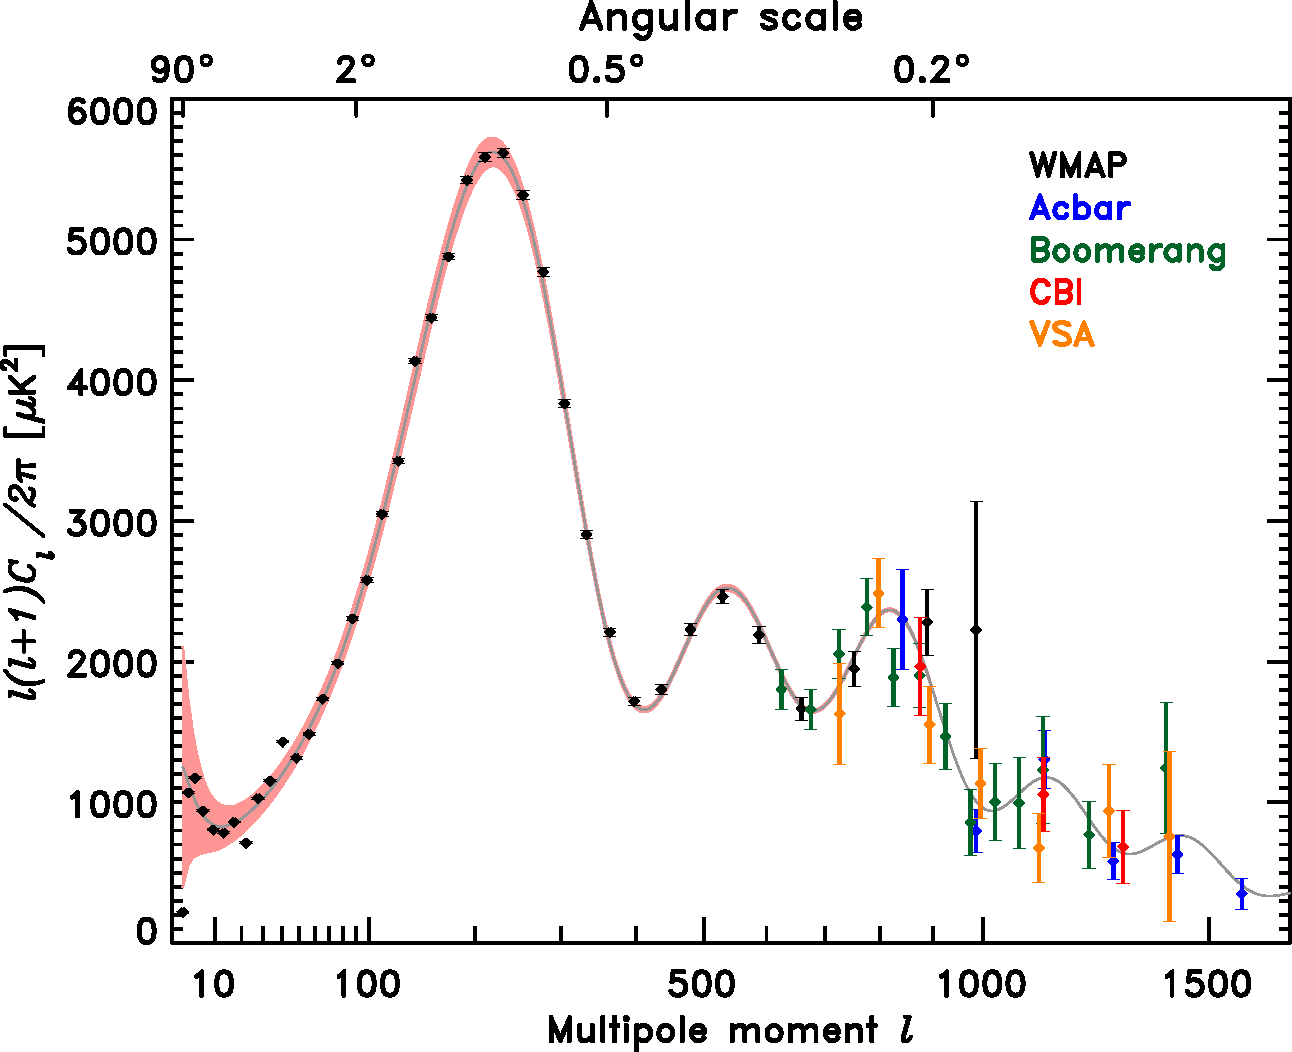
\includegraphics[width=\textwidth]{img/ch-03/power-spectrum.pdf}
	\caption{The power spectrum of the cosmic microwave background radiation temperature anisotropy in terms of the angular scale (or multipole moment). The measurements and the theoretical model are shown.}
	\label{fig:power-spectrum}
\end{marginfigure}
















